\documentclass[aspectratio=169]{beamer}
\usetheme{hogent}
\usecolortheme{hgwhite} % witte achtergrond, zwarte tekst

%% common.tex -- Code die in elk .tex-bestand terug komt

%% Packages

\usepackage[dutch]{babel}
\usepackage{graphicx}
\usepackage{comment,enumerate,hyperref}
\usepackage{amsmath,amsfonts,amssymb}
\usepackage{eurosym}
\usepackage{booktabs}
\usepackage{multicol,multirow}
\usepackage{listings}

\usepackage[outputdir=out]{minted}
%\usepackage{minted}

\usepackage[backend=biber,style=apa]{biblatex}
\DeclareLanguageMapping{dutch}{dutch-apa}

\usepackage{csquotes}

%% Variabelen, elk academiejaar aan te passen
\newcommand{\academicyear}{2023--2024 (revisie: \today)}
\newcommand{\lecturers}{Thomas Aelbrecht \and Thomas Parmentier \and Bert Van Vreckem}
\newcommand{\coursename}{Research Methods (IT)}

%% Macro's en commando's

%% \alertbox: een kader voor tekst die moet opvallen
\newcommand{\alertbox}[2][hgblue]{%
  \setbeamercolor{alertbox}{bg=#1,fg=white}
  \begin{beamercolorbox}[sep=2pt,center]{alertbox}
    \textbf{#2}
  \end{beamercolorbox}
}

\addbibresource{rm4-bibliografie.bib}

%---------- Info over de presentatie ------------------------------------------

\title{Module 4. Creating a bibliographic database.}
\subtitle{\coursename}
\author{\lecturers}   % Pas waarden aan in common.tex
\date{\academicyear}

\begin{document}

\begin{frame}
  \maketitle
\end{frame}

\begin{frame}
  \frametitle{Content}

  \tableofcontents
\end{frame}

\section{Literature study in {\LaTeX}.}

\begin{frame}
    \frametitle{Bibliografic database}
    
    \begin{itemize}
        \item = Software to store sources in a structured manner
        \item Full text + metadata
        \item Generate correctly styled literature list
        \item Reference management software
    \end{itemize}    
\end{frame}

\begin{frame}
    \frametitle{Examples}
    
    \begin{itemize}
        \item Endnote: commercial
        \item Mendeley: commercial, free
        \item JabRef: open source
    \end{itemize}
    
\end{frame}

\begin{frame}[plain]
    \frametitle{JabRef}
    
    \centering
    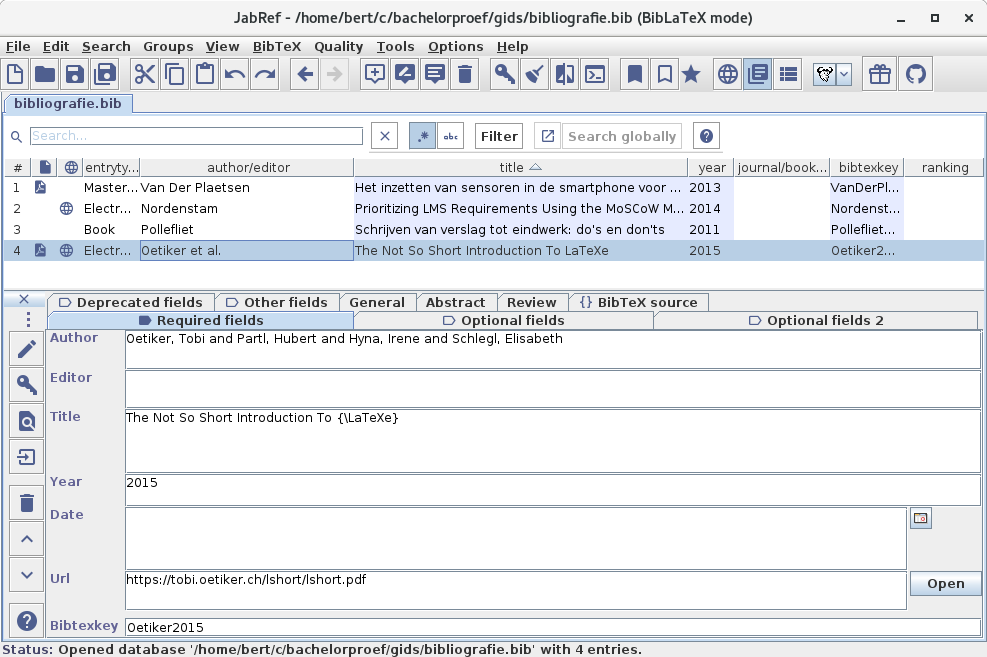
\includegraphics[height=.8\textheight]{4/jabref-screenshot}
    
\end{frame}

\begin{frame}
    \frametitle{JabRef settings}
    
    Options > Preferences
    
    \begin{itemize}
        \item General
        \begin{itemize}
            \item Default encoding: \textbf{UTF-8}
            \item Default library mode: \textbf{biblatex}
        \end{itemize}
        \item File
        \begin{itemize}
            \item Main file directory: (path to folder where you keep the PDF files)
        \end{itemize}
        \begin{itemize}
            \item Entry Preview: APA 7th edition
        \end{itemize}
    \end{itemize}
    
\end{frame}
\begin{frame}[fragile]
  \frametitle{Source citation and reference list in {\LaTeX}.}

  Bib{\LaTeX} and Biber

  \vspace{18pt}

  \verb|article.tex|: Main text\\
  \verb|article.bib|: Bibliografic database (edit using e.g.~JabRef)

  \bigskip

  Preamble:

  \begin{verbatim}
  \usepackage[backend=biber,style=apa]{biblatex}
  \DeclareLanguageMapping{dutch}{dutch-apa}
  \addbibresource{article.bib}
  \end{verbatim}

    \textbf{Remarl:}\ Already in template!
    
\end{frame}

\subsection{Creating a bibliographic database.}

\begin{frame}
  \frametitle{Bibliografic data in Jabref.}

  Fields that \textbf{always} need to be filled:

  \begin{description}
    \item[Author] Surname, Firstname and Surname, Firstname and Surname, Firstname \ldots
    \item[Title] of the article, book, \ldots
    \item[Year] or publication date
    \item[Bibtexkey] id of this source, used when referencing, (tip: click on the key icoon)
  \end{description}
    \bigskip
Impossible to fill in one of these fields? Then the source is probably unsuitable!
\end{frame}

\begin{frame}
    \frametitle{The author field}
    
    Always use this format:
    
    \begin{itemize}
        \item Persons: ``Surname, Firstname and Surname, Firstname and Surname, Firstname\ldots''
        \item Organisation: between curly brackets e.g.\ ``\{The Linux Foundation\}''
    \end{itemize}
    
\end{frame}

\begin{frame}[fragile]
  \frametitle{Bibliografic data in Jabref.}
  \framesubtitle{Extra fields for Article}

  \begin{description}
    \item[Journal] Name of the journal
    \item[Volume] Volume
    \item[Number] Number within the volume (optional)
    \item[Pages] \verb|mmm--nnn|
  \end{description}

  \bigskip

  \textbf{Example:} 

  \fullcitebib{Anscombe1973}
\end{frame}

\begin{frame}
    \frametitle{Tip: fill in fields automatically}
    
    \begin{itemize}
        \item Elsevier, Springer, \ldots\ have Bib\LaTeX{} export function
        \item Paste in tab page ``BibTeX source''
    \end{itemize}
    
    \bigskip
    
    \centering
    
\includegraphics[height=.6\textheight]{4/elsevier-cite-doi}
    
\end{frame}

\begin{frame}
    \frametitle{Tip: fill in fields automatically}
    
    \begin{itemize}
        \item DOI = Digital Object Identifier
        \item Unique code for a publication
        \item Jabref: General > DOI > Get Bibtex data from DOI
    \end{itemize}
    
    \bigskip
    
    \centering
    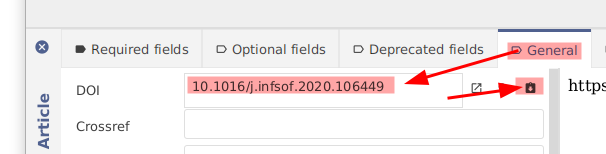
\includegraphics[height=.3\textheight]{4/jabref-doi}
    
\end{frame}

\begin{frame}[plain]
    \frametitle{Tip: fill in fields automatically}
    
    \centering
    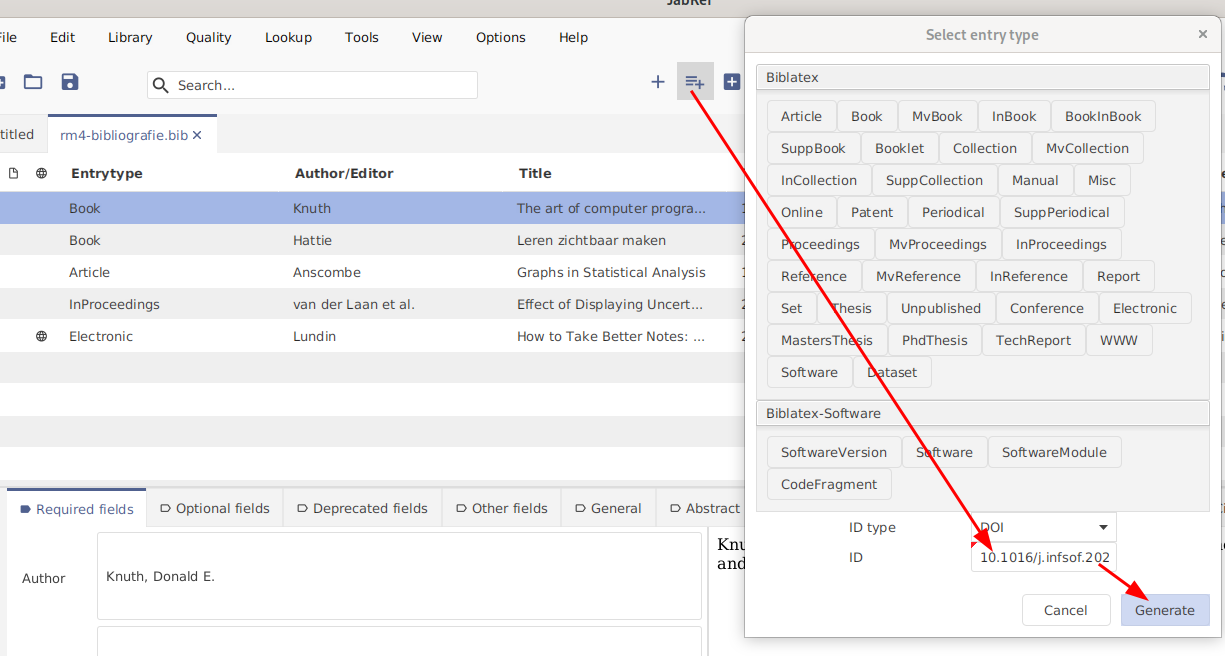
\includegraphics[height=.8\textheight]{4/jabref-new-entry-doi}
    
\end{frame}

\begin{frame}[plain]
  \frametitle{Bibliografic data in Jabref.}
  \framesubtitle{Extra fields for Electronic (Online, WWW)}

  \begin{description}
    \item[Url] Hyperlink to source
    \item[Urldate] Visit date
  \end{description}

  \bigskip

  \textbf{Example:}

  \bigskip

  \fullcitebib{Lundin2020}

\end{frame}

\begin{frame}[plain]
  \frametitle{Bibliografic data in Jabref.}
  \framesubtitle{Extra fields for InProceedings}

  \begin{description}
    \item[Booktitle] ``Proceedings of the [name conference]''
    \item[Editor] Editor(s) (optional)
    \item[Pages] Page numbers (optional)
  \end{description}

  \medskip

  \textbf{Example:}

  \fullcitebib{vanderLaanEtAl2015}
\end{frame}

\begin{frame}
  \frametitle{Bibliografic data in Jabref.}

  Fill out as much information as possible (facilitates searching):

  \begin{description}
    \item[DOI] Digital Object Identifier: unique ID for article, automatically fill in every field
    \item[URL] even if it is not a real Electronic source
    \item[Keywords] Keywords
    \item[File] PDF of the publication
    \item[Abstract] Summary
    \item[Comments] Your own summary/remarks
  \end{description}

\end{frame}

\section{Referencing literature.}

\begin{frame}[fragile]
    \frametitle{Referencing in the text}
    
    \begin{itemize}
      \item \verb|\textcite{Knuth1998}| \(\Rightarrow\) Knuth (1998)
      \item \verb|\autocite{Knuth1998}| \(\Rightarrow\) (Knuth, 1998)
    \end{itemize}
\end{frame}

\begin{frame}
\frametitle{Use \texttt{\textbackslash{}textcite}}

\ldots\ if the name of the author is part of the sentence:

\bigskip

\begin{quotation}
    An overview is provided in the survey by Ribas et al (2010). For a real-life case-study of applying genetic algorithm ``on top'' of a Mixed Integer Linear Programming model, we refer to Borodin et al (2011).
\end{quotation}

\end{frame}

\begin{frame}
\frametitle{Use \texttt{\textbackslash{}autocite}}

\ldots\ if the name of the author is NOT part of the sentence 

\bigskip

\begin{quotation}
    Reinforcement Learning (RL) is a technique that allows an agent to learn how to maximize a numerical reward signal (Sutton and Barto, 1998).
\end{quotation}

\bigskip

Also: exact citation, source of image 

\end{frame}


%% TODO: uitgewerkte voorbeelden! \textcite, \autocite, citaat, bijschrift afbeelding?

\begin{frame}[fragile]
\frametitle{Insert reference list.}

\begin{itemize}
    \item Insert reference list: \verb|\printbibliography|

    \item Compile (in TexStudio):

    \begin{enumerate}
      \item Build/Compile (F5): sources are not added yet, ``keys'' of sources are marked in bold
      \item Bibliography (F8): selects the referenced sources and prepares them 
      \item Build/Compile (F5): inserts references in the text and generates the reference list
    \end{enumerate}
  \end{itemize}
\end{frame}

\begin{frame}
 \frametitle{Check the result!}
  \begin{itemize}
     \item Authors correctly displayed?
     \item Language errors or typos? E.g.\ accents, special characters
     \item All info needed to find source is present?
     \item Mentioning of ``Visited DATE, of URL'' with Online sources?
     \item \ldots
 \end{itemize}
 \end{frame}

\begin{frame}
  \frametitle{Common mistakes}

  \begin{itemize}
    \item Non-scientific sources used (e.g.\ StackOverflow, Wikipedia, blogs not by a subject expert, \ldots)
    \item URLs not cleaned up (e.g. markers like \texttt{\#:$\sim$:text=something} in URL - Scroll To Text Fragment feature of browsers)
    \item Incorrect or missing information (e.g. missing page numbers, wrong order of authors, wrong author, \ldots)
    \item Incorrect citation type (e.g. \texttt{Online} instead of \texttt{Book} for a book - typically seen for books found via Google Books)
    \item \ldots
  \end{itemize}
\end{frame}

\begin{frame}[plain]
    \frametitle{Exercise}
    
    Save these sources in JabRef, with all necessary info and fulltext (where possible) and/or URL of the online source:
    
    \bigskip
    
    \begin{itemize}
        \item \url{https://www.sciencedirect.com/science/article/abs/pii/S0020025510002756}
        \item \url{https://catalogus.hogent.be/catalog/hog01:000617334}
        \item \url{https://martinfowler.com/articles/microservices.html}
        \item \url{https://www.youtube.com/watch?v=wW9CAH9nSLs&t=13s}
        \item \url{https://link.springer.com/book/10.1007/978-1-4842-6399-0}
        \item \url{http://www.schedulingconference.org/proceedings/2013/mista2013.pdf} (pp.\ 402--409)
        \item \url{https://docs.ansible.com/ansible-core/devel/index.html}
    \end{itemize}
    
\end{frame}

\begin{frame}
    \frametitle{Assignment}
    
    \begin{itemize}
        \item Save all found sources in .bib-file
        \item Structure, e.g.\ using Mind Map
        \begin{itemize}
            \item Freemind, Gitmind, Xmind, Minder, Vym, \ldots
        \end{itemize}
        \item Process what you read to a continuous text
    \end{itemize}
    
    \bigskip
    
    \alertbox{This is the most important phase of the assignment!}
\end{frame}

\end{document}
